\documentclass[conference]{IEEEtran}
\IEEEoverridecommandlockouts
% The preceding line is only needed to identify funding in the first footnote. If that is unneeded, please comment it out.
\usepackage{cite}
\usepackage{amsmath,amssymb,amsfonts}
\usepackage{algorithmic}
\usepackage{graphicx}
\usepackage{textcomp}
\usepackage{xcolor}
\usepackage{listings}
\usepackage{float}

\def\BibTeX{{\rm B\kern-.05em{\sc i\kern-.025em b}\kern-.08em
    T\kern-.1667em\lower.7ex\hbox{E}\kern-.125emX}}
\begin{document}

\title{A Brief Survey on RC4  Cryptography
}

\author{\IEEEauthorblockN{Prashanth A R}
\IEEEauthorblockA{\textit{Dept. of CSE} \\
\textit{PES University }\\
Bangalore, India \\
prashanthathunt@gmail.com}

}

\maketitle

\begin{abstract}
RC4 may be a stream cipher which was most generally accepted for its structural simplicity. it's high rate of encryption and decryption rate i.e speed and efficiency.
There were several reports on RC4 algorithm vulnerabilities and further proposals on modified RC4 algorithm. In spite of of these vulnerabilities still RC4 is been utilized in TSL web connections.
There were many efforts on removing weakness of RC4 like biased key , key collisions, key recovery etc , specifically from WEP ,so WPA standard was introduced to over come these vulnerabilities . WPA was again proved insecure due to TB data injection attack.researchers are performing on RC4 from past 20 years but still the attraction towards RC4 has been alive.
 
\end{abstract}

\begin{IEEEkeywords}
RC4 , cryptography , stream cipher , algorithm , survey  
\end{IEEEkeywords}



\section{Introduction}
RC4(Rivest Cipher 4) is additionally referred to as ARC4 or ARCFOUR meaning Alleged RC4. RC4 may be a stream cipher , which is understood for its simplicity and performance in software . RC4 became a neighborhood of encryption protocols and standards, like WEP in 1997 , in 2003 WPA was released for wireless cards , and in 1995 SSL  and its successor TLS in 1999 ,TLS and SSL was a great success  until it was prohibited in 2015 due to RC4 attack or cracking RC4 which was main cryptography used in SSL/TLS. RC4 was very easy to implementation on software and hardware devices.
RC4 may be a symmetric encryption where single key's shared between both the parties to encrypt and decrypt the cipher [1]
Secret key ciphers can be classified into 2 main branches  \newline a.stream ciphers \newline b. block ciphers.RC4 may be a Stream cipher which suggests it encryption takes palace bit by bit where as in block ciphers it the encryption will happen during a fixed size block.
The strength of the stream cipher depends on the random key stream generated which is then xor-ed with the plain text. 

\section{Algorithm}
RC4 algorithm has 2 main components KSA(Key-scheduling algorithm ) and PRGA(Pseudo-random generation algorithm) . the key key's passed though KSA and PRGA the output is bitwise xored with plaintext. it's almost like just one occasion pad expect that the pseudorandom number generated by PRGA is employed instead of prepared streams.



KSA is employed for initializing the S array , the output is given to PRGA.
\newline 
\newline 
\newline
\newline \newline \newline 
\newline 
\newline 
\centerline{KSA algorithm}

\begin{figure}[H]
    \centering
    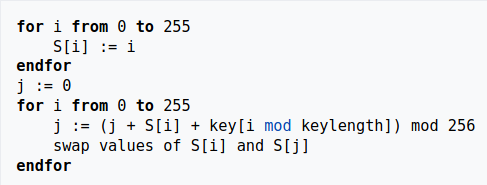
\includegraphics[width=\linewidth]{ksa}
    % \caption{Caption}
    % \label{fig:my_label}
\end{figure}

% \begin{verbatim}
% for i from 0 to 255
%     S[i] := i
% endfor
% j := 0
% for i from 0 to 255
%     j := (j + S[i] + key[i mod keylength]) mod 256
%     swap values of S[i] and S[j]
% endfor
% \end{verbatim}




For as many iterations as are needed, the PRGA modifies the state and outputs a byte of the keystream. In each iteration, the PRGA. \newline \newline

\centerline{PRGA algorithm}
\begin{figure}[H]
    \centering
    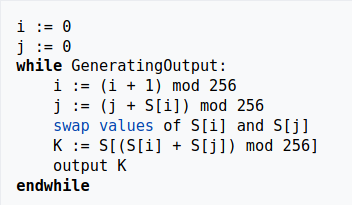
\includegraphics[width=\linewidth]{PRGA}
    % \caption{Caption}
    % \label{fig:my_label}
\end{figure}

% \begin{verbatim}
% i := 0
% j := 0
% while GeneratingOutput:
%     i := (i + 1) mod 256
%     j := (j + S[i]) mod 256
%     swap values of S[i] and S[j]
%     K := S[(S[i] + S[j]) mod 256]
%     output K
% endwhile
  
% \end{verbatim}

the output K stream is xored with the plaintext to encrypt the info , or it's xored with ciphertext to decrypt the info \newline \newline \newline \newline \newline \newline \newline \newline \newline \newline 

\begin{figure}[H]
    \centering
    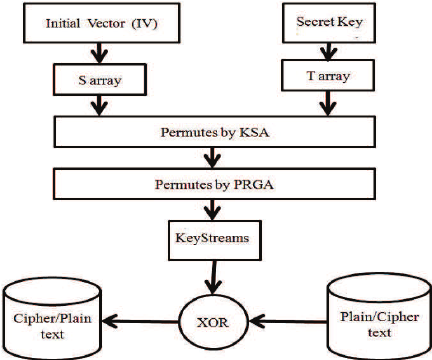
\includegraphics[width=\linewidth]{Encryption-and-decryption-by-RC4}
    \caption{RC4 flow diagram}
    \label{fig:my_label}
\end{figure}
%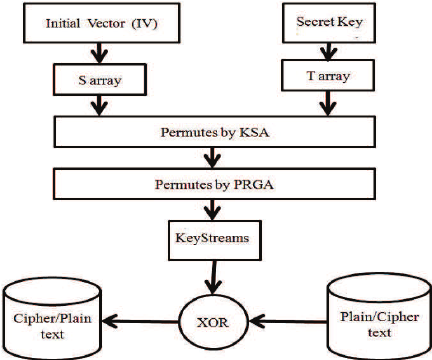
\includegraphics[scale=0.5]{Encryption-and-decryption-by-RC4}

\section{modification approaches}\newline
\newline
\newline


\centerline {PSEUDO CODE I} 
KSA OF IMPROVED RC4 PROPOSED BY JIAN XIE ET AL:[2].\newline \newline \newline

\begin{figure}[H]
    \centering
    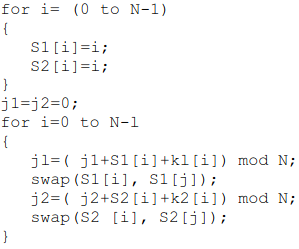
\includegraphics[width=\linewidth]{psudocode1}
    % \caption{Caption}
    % \label{fig:my_label}
\end{figure}\newline \newline 

% \begin{verbatim}
% for i = (0 to N-1) 
% {
%     S1[i]=i;
%     S2[i]=i;
% }
% j1=j2=0;
% for i = 0 to N-l 
% {
%     j1 = ( j1+S1[i]+kl[i]) mod N;
%     swap(S1[i], S1[j]);
%     j2=( j2+S2[i]+k2[i]) mod N;
%     swap(S2 [i], S2[j]);
% }    
% \end{verbatim}


\centerline{PSEUDO CODE II} 

PRGA OF IMPROVED RC4 PROPOSED BY JIAN XIE ET AL:[2].

\begin{figure}[H]
    \centering
    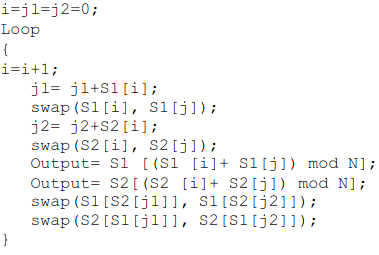
\includegraphics[width=\linewidth]{code2}
    % \caption{Caption}
    % \label{fig:my_label}
\end{figure}
% \begin{verbatim}
% i=j1=j2=0;
% Loop 
% {   
%     i=i+1;
%     j1= j1+S1[i];
%     swap(S1[i], S1[j]);
%     j2= j2+S2[i];
%     swap(S2[i], S2[j]); 
%     Output = S1  [(S1 [i]+ S1[j]) mod N];
%     Output= S2[(S2 [i]+ S2[j]) mod N];
%     swap(S1[S2[j1]], S1[S2[j2]]);
%     swap(S2[S1[j1]], S2[S1[j2]]);
% } 
% \end{verbatim}

\begin{figure}[H]
    \centering
    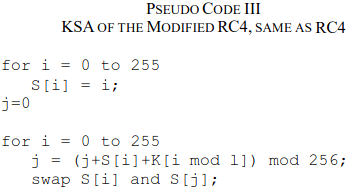
\includegraphics[width=\linewidth]{code3}
    % \caption{Caption}
    % \label{fig:my_label}
\end{figure}


\begin{figure}[H]
    \centering
    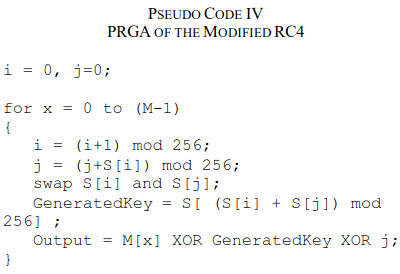
\includegraphics[width=\linewidth]{code4}
    % \caption{Caption}
    % \label{fig:my_label}
\end{figure}
Many more modification on RC4 are made in decades to improve security as well as speed . \newline
\begin{figure*}
    \centering
    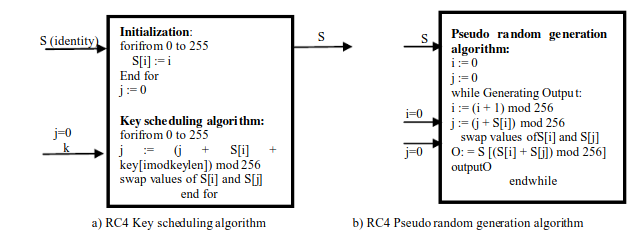
\includegraphics[width=\linewidth]{RC4}
    \caption{RC4}
    \label{fig:my_label}
\end{figure*}
%includegraphics[height=6cm , width=10cm]{RC4}

\section{SECURITY ANALYSIS}
\begin{itemize}
\item RC4 is mainly used  in WLAN security
protocols because of it performance and low computation power need. Wired equivalent privacy (WEP) is the primary security protocol used for Wi -Fi security in IEEE 802.11 LANs and is based  on RC4 encryption algorithm. due to the amount of attacks on WEP such as;
related key attacks[3], Fluhrer, Mantin and Shamir attack (FMS)[4], Korek practical attacks[5], Mantin attack on RC4 [6] and WEP,and many more therefore WEP was announced  as an insecure protocol.
WPA was more secure by defended against many attacks in WEP.

\item WPA has again announced to be a weak protocol due to TB data injection attacks[7], and SVV attacks[8]]. new
protocol WPA2 was announced which uses AES (type of symmetric cipher called Advance encryption standard which is a type of block cipher ) as an encryption algorithm
instead of RC4. Even Though WPA2 may be a secure protocol, removing many vulnerabilities of WEP.
hardware based applications which uses WEP and WPA with RC4 were cost effective.
\item Further a replacement protocol WPA2 was proposed by the WiFi alliance which uses AES block cipher as an standard encryption algorithm instead of RC4.
Though WPA2 could also be a secure protocol, removing many vulnerabilities of WEP and WPA but its hardware based applications are not  cost effective as compare to WEP and WPA where RC4 cryptography algorithm is used as a basis.

\item RC4 is additionally widely used and accepted in web security. it's utilized in Transport layer security (TLS) /SSL to supply security over the web . The RC4 is understood to the simplest choice for TLS/SSL because it can 
mitigate many attacks on the protocol. However recently in 2013 and 2014, a replacement security attack[9] on RC4 of
Although there has been many successful security breaches within the protocols using RC4, but the striking 
combination of style elegance and robustness of RC4 has made it most widely accepted protocol for last 20 years .  \newline \newline \newline\newline 
\end{itemize}
\begin{figure*}
    \centering
    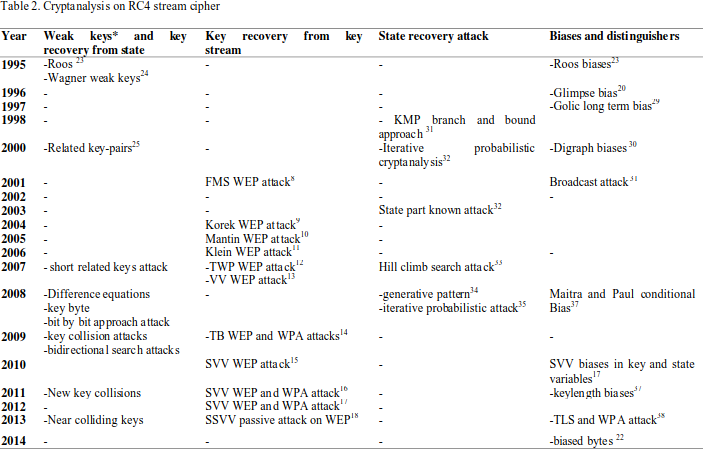
\includegraphics[width=\linewidth]{Screenshot_2020-09-21 (PDF) A Survey on RC4 Stream Cipher}
    \caption{list of known weakness of RC4}
    \label{fig:my_label}
\end{figure*}

\section{Application}
RC4 was widely utilized in WLAN connection in WEP and WPA . WPA2 uses AES for better security . RC4 was been utilized in TLS/SSL before 2015 which is not any more utilized in web security. versions of RC4 is employed in bluetooth , radios and lots of more small devices which has low computation power but yet security is vital 
There are many variant of RC4  like 
RC4A proposed by Bart Preneel and  Souradyuti Paul [10] \newline
Variably Modified Permutation Composition (VMPC) [11]\newline
Spritz by  Rivest, Ron; Schuldt, Jacob (27 October 2014)[12]. \newline
RC4+ by Goutam Paul and Subhamoy Maitra (19 September 2008)[13] \newline \newline \newline \newline \newline 

\section*{Conclusion}
In this article I even have presented a fast study of RC4
,about is robust feature and its weaknesses . How easy
it is to implement on hardware and software .I had
presented a wide kinds of RC4 algorithms improving the
security aspects of RC4 . it had been widely utilized in wireless
communication( like WEP and WPA) and web security like
TLS/SSL until it had been declared to be insecure . \newline
In spite of all the improvements / developments reported within the literature, there
are still many open research issues and challenges  related
to searches of more  key collisions in key stream, biases, and
key recovery attack on WPA .The conclusion is there's still
research happening , on RC4 to make it more efficient and
robust encryption algorithm.\newline \newline 
\section*{Acknowledgment}
Thanking the PES Institution and therefore the Teachers for his or her
support, Guidance and encouragement. \newline \newline 
\section*{References}
[1]Alfred J. Menezes, Paul C. van Oorschot, and Scott A.
Vanstone. Hand- book of Applied Cryptography. CRC Press,
August 2011 edition, 1996. Fifth Printing
\newline
[2] J. Xie, X. Pan, —An Improved RC4 Stream Cipher||,
2010 International Conference on Computer A pplication and
System Modeling, (ICCASM 2010), pp. (V7) 156-159, 2010
\newline
[3]Ronald L. Rivest. RSA security response to weaknesses in
key scheduling algorithm of RC4. Technical note, RSA Data
Security, Inc., 2001.
\newline
[4] Scott R. Fluhrer, Itsik Mantin, and Adi Shamir. Weaknesses
in the key scheduling algorithm of RC4. In Serge Vaudenay
and Amr M. Youssef, editors, Selected Areas in Cryptography,
volume 2259 of Lecture Notes in computing , p. 1–24.
Springer, 2001.
\newline
[5] Korek. Need security pointers. Published online at
http://www.netstumbler.org/showthread.php?postid=89036
\newline
[6] Itsik Mantin. A practical attack on the fixed RC4 within the
WEP mode. In Bimal K. Roy, editor, ASIACRYPT, volume
3788 of Lecture Notes in computing , p. 395–411.
Springer, 2005.
\newline
[7] Erik Tews and Martin Beck. Practical attacks against
WEP and WPA. In David A. Basin, Srdjan Capkun, and
Wenke Lee, editors, WISEC , p. 79–86. ACM, 2009
\newline
[8] Pouyan Sepehrdad, Serge Vaudenay, and Martin Vuagnoux.
Statistical attack on RC4 - distinguishi ng WPA. In Kenneth
G. Paterson, editor, EUROCR YPT, volume 6632 of Lecture
Notes in computing , p. 343–363. Springer, 2011
\newline
[9] Santanu Sarkar, Sourav Sen Gupta, Goutam Paul, and
Subhamoy Maitra. Proving TLS-attack related open biases of
RC4. IACR Cryptology ePrint Archive, 2013:502, 2013.
\newline
[10]Souradyuti Paul; Bart Preneel (2004), ”A New Weakness
in the RC4 Keystream Generator and an Approach to enhance
the Security of the Cipher”, Fast Software Encryption, FSE
2004, Lecture Notes in computing , 3017, Springer-
Verlag, pp. 245–259, doi:10.1007/978-3-540-25937-4 16,
ISBN 978-3-540-22171-5, retrieved 4 November 2011
\newline
[11]Bartosz Zoltak (2004), ”VMPC One-Way Function
and Stream Cipher” (PDF), Fast Software Encryption,
FSE 2004 (PDF), Lecture Notes in computing ,
3017, Springer-Verlag, pp. 210–225, CiteSeerX
10.1.1.469.8297,doi:10.1007/978-3-540-25937-4 14, ISBN
978-3-540-22171-5, retrieved 4 November 2011
\newline
[12]Rivest, Ron; Schuldt, Jacob (27 October 2014). ”Spritz –
a spongy RC4-like stream cipher and hash function” (PDF).
Retrieved 26 October 2014
\newline
[13]Subhamoy Maitra; Goutam Paul (19 September 2008),
”Analysis of RC4 and Proposal of Additional Layers for Better
Security Margin”, Progress in Cryptology – INDOCRYPT
2008 (PDF), Lecture Notes in computing , 5365,
Springer-Verlag, pp. 27–39, CiteSeerX 10.1.1.215.7178,
doi:10.1007/978-3-540-89754-5 3, ISBN 978-3-540-89753-8,
Cryptology ePrint Archive: Report 2008/396, retrieved 4
November 2011

\end{document}

